\chapter{Integration in $\R^{\lowercase{n}}$}
Im Eindimensionalen hatten wir mit dem Integral \[\int\limits_a^b f(x)dx\] den Flächeninhalt unter dem Graphen von $f$ berechnet. Wir suchen nach einer Verallgemeinerung mit der \todo{can't understand word, page 207 middle} z.B. Volumen unter dem Graphen einer Funktion von zwei Variablen berechnet werden kann.


\begin{multicols}{2}
\begin{center}
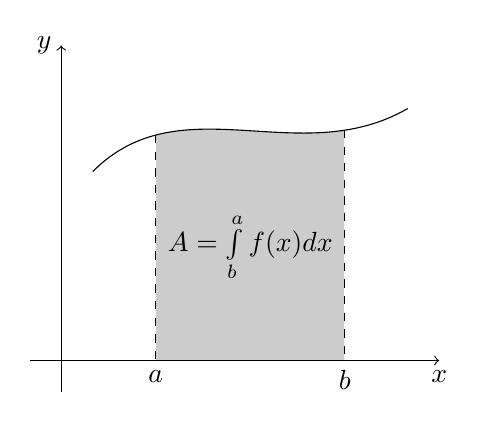
\begin{tikzpicture}[scale=0.8]
\shade[top color=black!20,bottom color=black!20,in=-150, out=45] 
      (0.5,3) to (5.5,4) |- (0.5,0);
\draw[fill=white,color=white] (0.5,5) -- (1.5,5) -- (1.5,0)--(0.5,0)--cycle;
\draw[fill=white,color=white] (4.5,5) -- (6,5) -- (6,0)--(4.5,0)--cycle;

\draw[->] (-0.5,0)--(6,0) node [anchor=north]{$x$};;
\draw[->] (0,-0.5)--(0,5) node [anchor=east]{$y$};
\draw [in=-150, out=45] (0.5,3) to (5.5,4);
\draw[dashed] (1.5,3.58)--(1.5,0) node [anchor=north]{$a$};
\draw[dashed] (4.5,3.66)--(4.5,0) node [anchor=north]{$b$};
\draw (3,1.8) node {$A=\int\limits^a_b f(x)dx$};
\end{tikzpicture}
\end{center}
\columnbreak
\begin{center}
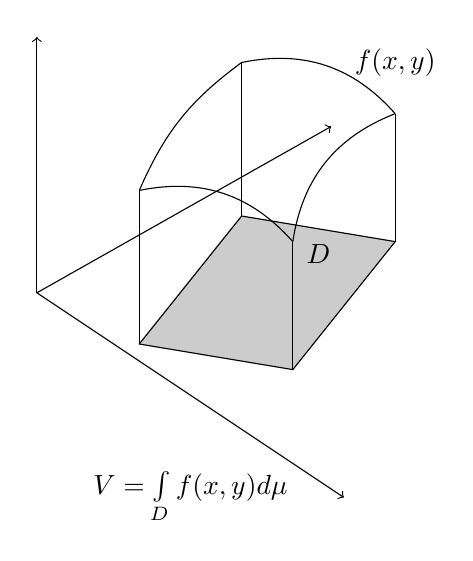
\begin{tikzpicture}[scale=0.65]
		\node [] (0) at (0, 0) {};
		\node [] (1) at (5.75, 3.25) {};
		\node [] (2) at (6, -4) {};
		\node [] (3) at (0, 5) {};
		\node [] (4) at (2, -1) {};
		\node [] (5) at (4, 1.5) {};
		\node [] (6) at (5, -1.5) {};
		\node [] (7) at (7, 1) {};
		\node [] (8) at (2, 2) {};
		\node [] (9) at (4, 4.5) {};
		\node [] (10) at (7, 3.5) {};
		\node [] (11) at (5, 1) {};
		
\draw[fill=black!20, color=black!20] (4.center) -- (5.center) -- (7.center) -- (6.center)-- cycle;

		\draw [->] (0.center) to (3.center);
		\draw [->] (0.center) to (1.center);
		\draw [->] (0.center) to (2.center);
		\draw [] (4.center) to (6.center);
		\draw [] (4.center) to (5.center);
		\draw [] (5.center) to (7.center);
		\draw [] (7.center) to (6.center);
		\draw [] (4.center) to (8.center);
		\draw [] (5.center) to (9.center);
		\draw [] (7.center) to (10.center);
		\draw [] (6.center) to (11.center);
		\draw [, bend left] (8.center) to (11.center);
		\draw [, bend left] (11.center) to (10.center);
		\draw [, bend right] (10.center) to (9.center);
		\draw [, bend right=15] (9.center) to (8.center);
\draw (5.5,0.75) node {$D$};
\draw (7,4.5) node {$f(x,y)$};
\draw (3,-4) node {$V=\int\limits_D f(x,y)d\mu$};
\end{tikzpicture}
\end{center}
\end{multicols}



\underline{Erinnerung:} Das bestimmte Riemann-Integral einer Funktion $f(x)$ über einem Intervall ist $\lbrack a,b\rbrack:$
\[I=\int\limits_a^b f(x)dx\] Das Integral $I$ war als Grenzwert der Riemannschen Ober- und Untersumme definiert (falls diese Grenzwerte jeweils existieren und übereinstimmten).\\

Das Konstruktionsprinzip für Bereichsintegrale ist analog. Aber der Definitionsbereich $D$ ist komplizierter. Wir betrachten zunächst den Fall zweier Variablen, $n=2$, und einen Definitionsbereich $D\subset\R^2$ der Form
\[D=\lbrack a_1,b_1\rbrack\times\lbrack a_2,b_2\rbrack\subset\R^2\]
d.h. $D$ ist ein kompakter Quader (Rechteck). Sei $f:D\to\R$ eine beschränkte Funktion.

\begin{definition}{9.1}
Mann nennt $Z=\left\{ \left( x_0,x_1,\dots,x_n\right), \left( y_0,y_1,\dots,y_m\right)\right\}$ eine Zerlegung des Quaders $D=\lbrack a_1,b_1\rbrack\times\lbrack a_2,b_2\rbrack$ falls gilt
\begin{align*}
a_1&=x_0 < x_1\dots <x_n=b_1\\
a_2&=y_0 < y_1\dots <y_m=b_2
\end{align*}
\begin{enumerate}
\item WHERE IS NUMBER 1??
\item Die Feinheit einer Zerlegung $Z\in Z\left( D\right)$ ist \[\left\| Z \right\|: = \mathop {\max }\limits_{i,j} \left\{ {\left| {{x_{i + 1}} - {x_i}} \right|,\left| {{y_{j + 1}} - {y_j}} \right|} \right\}\]
\item Für eine vorgegebene Zerlegung $Z$, nennt man die Mengen \[{Q_{ij}}: = \left[ {{x_i},{x_{i + 1}}} \right] \times \left[ {{y_j},{y_{j + 1}}} \right]\] die Teilquader der Zerlegung $Z$. Das Volumen des Teilquaders $Q_{ij}$ ist \[\text{vol}\left( {{Q_{ij}}} \right): = \left( {{x_{i + 1}} - {x_i}} \right)\left( {{y_{j + 1}} - {y_j}} \right)\]
\item Für beliebige Punkte $\xi_{ij}\in Q_{ij}$ der jeweiligen Teilquader nennt man \[{R_f}\left( Z \right): = \sum\limits_{i,j} {f\left( {{\xi _{ij}}} \right){\text{vol}}\left( {{Q_i}j} \right)} \] eine Riemannsche Summe zur Zerlegung $Z$
\item Analog zum Integral einer Variablen heissen für eine Zerlegung $Z$
\begin{align*}
{U_f}\left( Z \right): =&\sum\limits_{i,j} {\mathop {\inf }\limits_{\Romanbar{X}\in Q_{ij}} } f\left(\Romanbar{X}\right){\text{vol}}\left( {{Q_i}j} \right)\\
{O_f}\left( Z \right): =&\sum\limits_{i,j} {\mathop {\sup }\limits_{\Romanbar{X}\in Q_{ij}} } f\left(\Romanbar{X}\right){\text{vol}}\left( {{Q_i}j} \right)
\end{align*}
die Riemannsche Untersumme bzw. Riemannsche Obersumme von $f\left( x\right)$
\end{enumerate}
\end{definition}
\subsubsection*{Bemerkung 9.2}
\begin{enumerate}
\item Es gilt \[U_f\left( Z\right)\leq R_f\left( Z\right)\leq O_f\left( Z\right)\] d.h. eine Riemannsche Summe zur Zerlegung $Z$ liegt stets zwischen der Unter und Obersumme dieser Zerlegung.
\item Entsteht eine Zerlegung $Z_2$ aus der Zerlegung $Z_1$ durch Hinzunahme weiterer Zwischenpunkte $x_i$ und/oder $y_j$, so gilt
\begin{align*}
U_f\left( Z_2\right)&\geq U_f\left( Z_1\right)\text{ und }\\
O_f\left( Z_2\right)&\leq O_f\left( Z_1\right)
\end{align*}
Für zwei beliebige Zerlegungen $Z_1,Z_2$ gilt stets \[U_f\left( Z_1\right)\leq O_f\left( Z_2\right)\]

\begin{center}
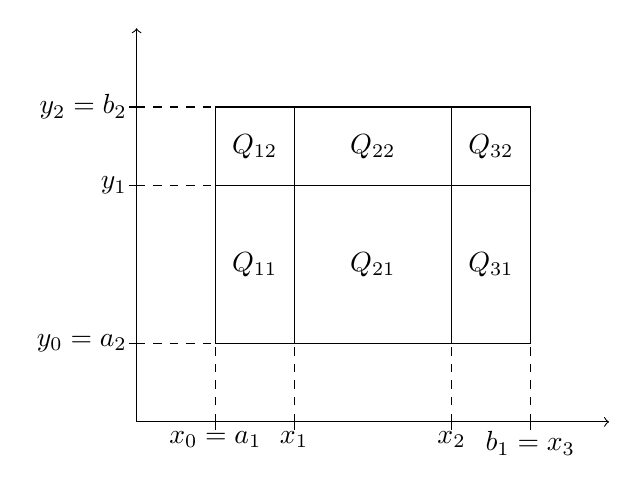
\begin{tikzpicture}[]

\draw[->] (0,0) --(6,0);
\draw[->] (0,0) --(0,5);

\draw (1,1) rectangle (5,4);

\draw[] (2,1) --(2,4);
\draw[dashed] (2,0)--(2,1);
\draw[] (4,1) --(4,4);
\draw[dashed] (4,0)--(4,1);
\draw[dashed] (1,0)--(1,1);
\draw[dashed] (5,0)--(5,1);

\draw[dashed] (0,1)--(1,1);
\draw[dashed] (0,3)--(1,3);
\draw[dashed] (0,4)--(1,4);

\draw (1,-0.1) -- (1,0) node [anchor=north]{$x_0=a_1$};
\draw (2,-0.1) -- (2,0) node [anchor=north]{$x_1$};
\draw (4,-0.1) -- (4,0) node [anchor=north]{$x_2$};
\draw (5,-0.1) -- (5,0) node [anchor=north]{$b_1=x_3$};

\draw (-0.1,1) -- (0,1) node [anchor=east]{$y_0=a_2$};
\draw (-0.1,3) -- (0,3) node [anchor=east]{$y_1$};
\draw (-0.1,4) -- (0,4) node [anchor=east]{$y_2=b_2$};

\draw[] (1,3) --(5,3);

\draw (1.5,2) node {$Q_{11}$};
\draw (3,2) node {$Q_{21}$};
\draw (4.5,2) node {$Q_{31}$};

\draw (1.5,3.5) node {$Q_{12}$};
\draw (3,3.5) node {$Q_{22}$};
\draw (4.5,3.5) node {$Q_{32}$};


\end{tikzpicture}
\end{center}

\end{enumerate}
\begin{definition}{9.3}
Sei $f:D\to\R$ beschränkt
\begin{enumerate}
\item Das Riemannsche Unterintegral bzw. Riemannsche Oberintegral der Funktion $f\left( x\right)$ über $D$ ist
\begin{align*}
{U_f}&: = \sup \left\{ {{U_f}\left( z \right):z \in Z\left( D \right)} \right\}: = \int\limits_{\underline{D}} {f(x)d\mu } \\
{O_f}&: = \inf \left\{ {{O_f}\left( z \right):z \in Z\left( D \right)} \right\}: = \int\limits_D^ -  {f(x)d\mu }
\end{align*}
\item Die Funktion $f(x)$ nennt man Riemann - integrierbar über $D$, falls Unter und Oberintegral übereinstimmen. Das Riemann Integral von $f(x)$ über $D$ ist \[\int\limits_D {f(x)d\mu  = \int\limits_D^ -  {f(x)d\mu  = } \int\limits_{\underline{D}} {f(x)d\mu } } \]
\end{enumerate}
\end{definition}

\subsubsection*{Bemerkung}
In höheren Dimensionen, $n >2$, ist die Vorgehensweise analog. Schreibweise: Für $n=2$, $n=3$
\[\int\limits_D {f\left( {x,y} \right)d\mu {\text{ bzw. }}} \int\limits_D {f\left( {x,y,z} \right)d\mu } \]
oder auch
\[\int\limits_D {f\left( {x,y} \right)dxdy{\text{ bzw. }}} \int\limits_D {f\left( {x,y,z} \right)dxdydz} \]
oder
\[\int\limits_D {fdxdy{\text{ bzw. }}} \int\limits_D {fdxdydz} \]

\subsubsection*{Satz 9.4 (Elementare Eigenschaften des Integrals)}
\begin{enumerate}
\item \underline{Linearität:} Seien $f,g: D\to\R$ beschränkt und R integrabel, $\alpha,\beta\in\R$. Dann sind $\alpha f$, $f+g$ Riemann-Integrabel
\[\int\limits_D {\left( {\alpha f + \beta g} \right)d\mu  = \alpha \int\limits_D {fd\mu }  + \beta \int\limits_D {gd\mu } } \]
\item \underline{Monotonie:} Gilt $f(x)\leq g(x)$, $\forall x\in D$, so folgt \[\int\limits_D {fd\mu }  \le \int\limits_D {gd\mu } \]
\item\underline{Positivität:} Gilt für alle $x\in D$, $f(x)\geq 0$ (d.h. $f(x)$ ist nicht negativ), so folgt \[\int\limits_D {fd\mu }  \ge 0\]
\item \underline{Abschätzung} \[\left| {\int\limits_D {f(x)d\mu } } \right| \le \mathop {\sup }\limits_{x \in D} \left| {f(x)} \right|{\text{vol}}\left( D \right)\]
\item Sind $D_1,d_2,D$ Quader, $D=D_1\cup D_2$ und $\text{vol}\left( D_1\cap D_2\right)=0$, so ist $f$ genau dann über $D$ integrierbar, falls $f$ über $D_1$ und über $D_2$ integrierbar ist und es gilt \[\int\limits_D {fd\mu }  = \int\limits_{{D_1}} {fd\mu }  + \int\limits_{{D_2}} {fd\mu } \](Gebietsadditivität)
\end{enumerate}

\section{Der Satz von Fubini}
\todo[inline]{According to the notes it should be 9.2, which one is right??}
Wie kann man das Riemann-Integral konkret berechnen? Der Satz von Fubini hilft uns.

\subsubsection*{Satz 9.5 (Satz von Fubini)}
Sei $Q=\lbrack a,b\rbrack\times \lbrack c,d\rbrack\in\R^2$ und sei $f\in C^0\left( Q\right)$. Dann gilt \[\int\limits_Q {fd\mu }  = \int\limits_a^b {\left( {\int\limits_c^d {f\left( {x,y} \right)dy} } \right)dx = \int\limits_c^d {\left( {\int\limits_a^b {f\left( {x,y} \right)dx} } \right)dy} } \]
d.h. das Integral von $f$ über $Q$ kann iterativ durch $1-$dimensionale Integration bestimmt werden.

\subsubsection*{Beispiel 9.6}
\begin{enumerate}
\item Sei $f\left( x,y\right)=2x+2yx$, $Q=\lbrack 0,1\rbrack\times\lbrack -2,2\rbrack$
\begin{align*}
\int\limits_Q {fd\mu }  =&\int\limits_{ - 2}^2 {\left( {\int\limits_0^1 {\left( {2x + 2yx} \right)dx} } \right)dy} \\
=&\int\limits_{ - 2}^2 {\left( {\left. {{x^2} + y{x^2}} \right|_0^1} \right)dy} \\
=&\int\limits_{ - 2}^2 {\left( {1 + y} \right)dy}  = \left. {y + \frac{{{y^2}}}{2}} \right|_{ - 2}^2 = 4
\end{align*}
\underline{Oder:}
\begin{align*}
&\int\limits_0^1 {\left( {\int\limits_{ - 2}^2 {\left( {2x + 2yx} \right)dy} } \right)dx} \\
 =&\int\limits_0^1 {\left( {\left. {2xy + {y^2}x} \right|_{ - 2}^2} \right)dx} \\
 =&\int\limits_0^1 {\left[ {\left( {4x + 4x} \right) - \left( { - 4x + 4x} \right)} \right]dx} \\
 =&\int\limits_0^1 {8xdx}  = \left. {4{x^2}} \right|_0^1 = 4
\end{align*}
\item \begin{align*}
&\int\limits_0^1 {\int\limits_0^{2\pi } {\left( {{e^x}\sin y} \right)dy} dx} \\
=&\int\limits_0^1 {\left( {\left. { - {e^x}\cos y} \right|_0^{2\pi }} \right)dx} \\
=&\int\limits_0^1 0 dx = 0
\end{align*}
\underline{Oder:}
\begin{align*}
&\int\limits_0^{2\pi } {\left( {\int\limits_0^1 {{e^x}\sin ydx} } \right)dy} \\
=&\int\limits_0^{2\pi } {\left( {\left. {\sin y{e^x}} \right|_0^1} \right)dy} \\
=&\int\limits_0^{2\pi } {\left( {e - 1} \right)\sin ydy} \\
=&\left. { - \left( {e - 1} \right)\cos y} \right|_0^{2\pi } = 0
\end{align*}
\end{enumerate}

\subsection*{Geometrische Deutung}\todo{Not sure about the text size...}
\begin{center}
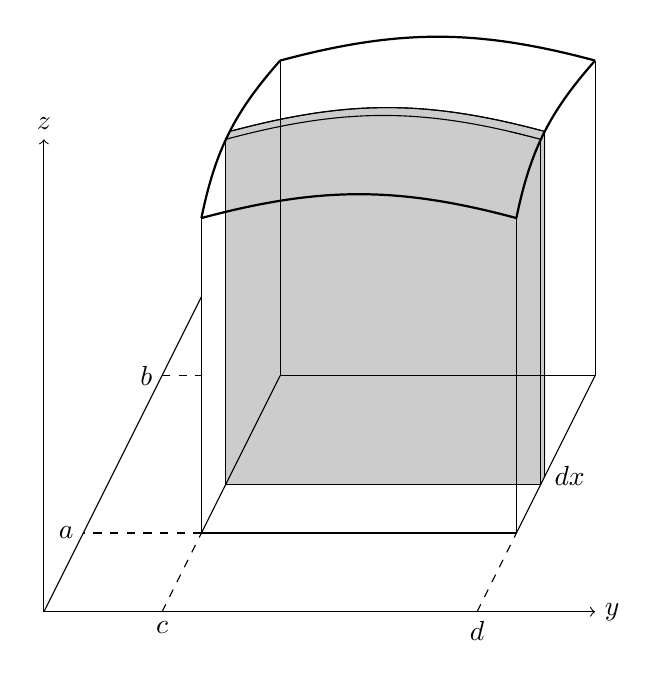
\begin{tikzpicture}
%Gray Sheet
\draw[color=black!20,fill=black!20] (0.31,5) -- (0.31,0.62) -- (4.31,0.62)  -- (4.31,5)--(0.31,5);
\draw [color=black!20,fill=black!20] (4.31,5)--(4.31,0.62)--(4.36,0.72)--(4.36,5.1) -- (4.31,5);
\draw [bend left=15,fill=black!20] (0.31,5) to (4.31,5);
\draw [bend left=15,fill=black!20] (0.36,5.1) to (4.36,5.1);
\draw[color=black!20,fill=black!20] (4.31,5) -- (4.36,5.1) -- (4,5.1) -- cycle; 
\draw[color=black!20,fill=black!20] (0.31,5) -- (0.36,5.1) -- (4,5.1) -- cycle; 

\node [] (0) at (0, 0) {};
\node [] (1) at (4, 0) {};
\node [] (2) at (5, 2) {};
\node [] (3) at (1, 2) {};
\node [] (4) at (0, 4) {};
\node [] (5) at (4, 4) {};
\node [] (6) at (5, 6) {};
\node [] (7) at (1, 6) {};
\node [] (8) at (-2, -1) {};
\node [] (9) at (5, -1) {};
\node [] (10) at (-2, 5) {};
\node [] (11) at (0, 3) {};
\node [] (12) at (-0.5, -1) {};
\node [] (13) at (3.5, -1) {};
\node [] (14) at (-1.5, 0) {};
\node [] (15) at (-0.5, 2) {};
\node [] (16) at (0, 2) {};
\draw [] (0.center) to (1.center);
\draw [] (1.center) to (2.center);
\draw [] (2.center) to (3.center);
\draw [] (3.center) to (0.center);
\draw [] (0.center) to (4.center);
\draw [thick, bend left=15] (4.center) to (5.center);
\draw [] (5.center) to (1.center);
\draw [] (3.center) to (7.center);
\draw [] (2.center) to (6.center);
\draw [thick, bend left=15] (4.center) to (7.center);
\draw [thick, bend left=15] (5.center) to (6.center);
\draw [thick, bend right=15] (6.center) to (7.center);
\draw [->, in=180, out=0] (8.center) to (9.center) node [anchor=west]{$y$};
\draw [->] (8.center) to (10.center) node [anchor=south]{$z$};
\draw [] (8.center) to (11.center);
\draw [dashed] (15.center) to (16.center);
\draw [dashed] (12.center) to (0.center);
\draw [dashed] (0.center) to (14.center) node [anchor=east]{$a$};
\draw [dashed] (13.center) to (1.center);
 \draw(13.center) node [anchor=north]{$d$};
 \draw(15.center) node [anchor=east]{$b$};
 \draw(-0.5,-1) node [anchor=north]{$c$};
\draw(4.36,0.72) node [anchor=west]{$dx$};








%Gray sheet limits
\draw [bend left=15] (0.31,5) to (4.31,5);
\draw [bend left=15] (0.36,5.1) to (4.36,5.1);
\draw [](0.31,5) -- (0.31,0.62);
\draw [](4.31,5) -- (4.31,0.62);
\draw [](4.36,5.1) -- (4.36,0.72);
\draw [](4.31,0.62) -- (0.31,0.62);
\end{tikzpicture}
\end{center}
In der Skizze ergibt sich als Volumen der markierten Schicht bei festem $x$ und sehr kleinen Dicke $dx$ näherungsweise das Volumen \[\left( {\int\limits_c^d {f\left( {x,y} \right)dy} } \right)dx\] Das Aufaddieren sämtlicher Schichtvolumen entspricht gerade der Integration über die Variable $x$, d.h. für das gesuchte Volumen gilt \[V = \int\limits_a^b {\left( {\int\limits_c^d {f\left( {x,y} \right)dy} } \right)dx} \]
Bis jetzt können wir nur Integrale über achsenparallel rechteckige bzw. quaderförmige Bereiche berechnen.\\

Das reicht für viele praktische Aufgaben nicht aus. Meist ist der Integrationsbereich $D$ verbogen oder zumindest anders begrenzt.
\missingfigure{Page 219 middle}
Die meisten praktischen Aufgaben lassen sich auf die Integration über sogenannte Normalbereiche zurückführen.

\begin{definition}{9.10}
\begin{enumerate}
\item Eine Teilmenge $D\subset\R^2$ heisst ein Normalbereich bezüglich der $x-$Achse bzw. bezüglich der $y-$Achse falls es stetige Funktionen $g,h$ bzw. $\overline{g},\overline{h}$ gibt mit
\[D=\left\{ \left( x,y\right)\mid a\leq x\leq b,\text{ und }g(x)\leq y\leq h(x)\right\}\]
bzw.
\[D=\left\{ \left( x,y\right)\mid \overline{a}\leq x\leq \overline{b},\text{ und }\overline{g}(x)\leq y\leq \overline{h}(x)\right\}\]
\end{enumerate}
\end{definition}

\subsubsection*{Beispiel}
Kreise und Rechtecke sind Normalbereiche bzgl. beider Achsen
\missingfigure{page 220 top; ALREADY STARTED, PICTURE ON THE RIGHT GETS PUSHED DOWN FOR SOME REASON, STILL TO FIX!}
%\begin{multicols}{2}
%\begin{tikzpicture}[scale=0.6]
%\draw[->] (-0.5,0)--(7,0) node [anchor=west] {$x$};
%\draw[->] (0,-0.5)--(0,6) node [anchor=south] {$y$};
%\draw[fill=black!20] (1,1)parabola bend (1,1)(6,5) parabola bend (1,3)(1,3) -- (1,1);
%\draw (3.1,3.7) node [anchor=south] {$y=h(x)$};
%\draw (4.2,1) node [anchor=south] {$y=g(x)$};
%\draw[dashed] (6,5) -- (6,0) node [anchor=north] {$b$};
%\draw[dashed] (1,1) -- (1,0) node [anchor=north] {$a$};
%\end{tikzpicture}
%\columnbreak
%\begin{tikzpicture}[scale=0.5]
%		\node [] (0) at (1, 1) {};
%		\node [] (1) at (1, 5) {};
%		\node [] (2) at (6, 5) {};
%		\node [] (3) at (6, 3.5) {};
%		\node [] (4) at (6, 1) {};
%		\draw[fill=black!20]  (0.center) .. controls (2,3) and (2,3) .. (1.center) -- (2.center) .. controls (5.5,4.25) and (5.5,4.25) .. (3.center) .. controls (6.75,2.25) and (6.75,2.25) .. (4.center)--cycle;
%\draw[->] (-0.5,0) -- (8,0) node [anchor=west] {$x$};
%\draw[->] (0,-0.5) -- (0,7.15) node [anchor=south] {$y$};
%\draw[dashed] (0,1)--(1,1);
%\draw[dashed] (1,5) -- (0,5);
%\draw (0,1) node[anchor=east] {$\overline{a}$};
%\draw (0,5) node[anchor=east] {$\overline{b}$};
%\draw (0.4,4) node[anchor=west]{$x$};
%\draw (0.3,3.5) node[anchor=west]{$=$};
%\draw (0.1,2.9) node[anchor=west]{$\overline{g}(y)$};
%\draw (6.5,3) node[anchor=west]{$x=\overline{h}(y)$};
%\end{tikzpicture}
%\end{multicols}
Über Normalbereiche lässt sich sehr bequem integrieren
\missingfigure{Page 220 bottom}
Die markierte Scheibe bei $y=$const. mit kleiner Dicke $dx$ besitzt näherungsweise das Volumen
\[V(x) = \left( {\int\limits_{g(x)}^{f(x)} {f\left( {x,y} \right)dy} } \right)dx\]
Nun braucht man $V(x)$ nur noch über $\lbrack a,b\rbrack$ zu integrieren\[V = \int\limits_a^b {\left( {\int\limits_{g(x)}^{h(x)} {f\left( {x,y} \right)dy} } \right)dx} \]

\subsubsection*{Satz 9.11}
\begin{enumerate}
\item Ist $f(x)$ stetig auf einem Normalbereich \[D=\left\{ \left( x,y\right)\in\R^2\mid a\leq x\leq b,\text{ und }g(x)\leq y\leq h(x)\right\}\]
so gilt
\[\int\limits_D {f(x)d\mu  = \int\limits_a^b {\left( {\int\limits_{g(x)}^{h(x)} {f\left( {x,y} \right)dy} } \right)dx} } \]
\item bzw. falls \[D=\left\{ \left( x,y\right)\in\R^2\mid \overline{a}\leq x\leq \overline{b},\text{ und }\overline{g}(x)\leq y\leq \overline{h}(x)\right\}\]
so gilt
\[\int\limits_D {f(x)d\mu  = \int\limits_{\overline{a}}^{\overline{b}} {\left( {\int\limits_{\overline{g}(x)}^{\overline{h}(x)} {f\left( {x,y} \right)dx} } \right)dy} } \]
\end{enumerate}
\subsubsection*{Beispiel 9.12}
\begin{enumerate}
\item Sei $f\left( x,y\right)=x-y$

\begin{center}
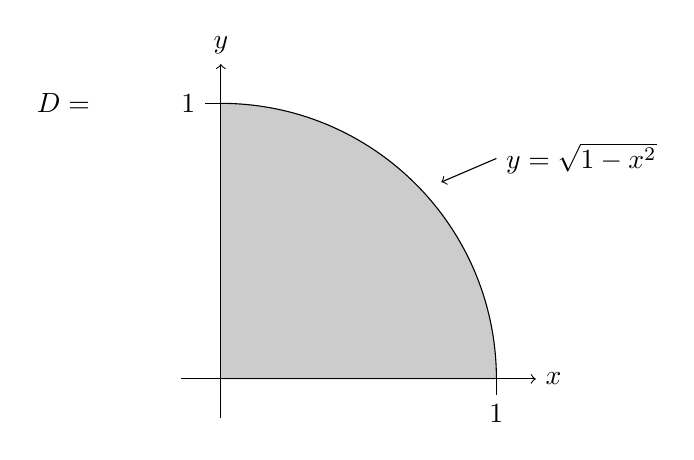
\begin{tikzpicture}[scale=1]

\draw[color=black!20,fill=black!20] (0,0)--(3.5,0)--(0,3.5)--cycle;

\draw[->] (-0.5,0) --(4,0) node [anchor=west]{$x$};
\draw[->] (0,-0.5) --(0,4) node [anchor=south]{$y$};;

\draw[fill=black!20] (3.5,0) arc (0:90:3.5);

\draw (3.5,0.05)--(3.5,-0.2) node [anchor=north] {1};
\draw (0.05,3.5)--(-0.2,3.5) node [anchor=east] {1};

\draw[<-] (2.8,2.5) -- (3.5,2.8)node [anchor=west]{$y=\sqrt{1-x^2}$};

\draw (-2,3.5) node {$D=$};
\end{tikzpicture}
\end{center}

\begin{align*}
\int\limits_D fd\mu =&\int\limits_{x=0}^{x=1}\int\limits_{y=0}^{y=\sqrt{1-x^2}}\left( x-y\right) dy dx\\
 =&\int\limits_0^1 {\left( {\left. {xy - \frac{{{y^2}}}{2}} \right|_0^{\sqrt {1 - {x^2}} }} \right)} dx\\
=&\int\limits_0^1 {\left( {x\sqrt {1 - {x^2}}  - \frac{{1 - {x^2}}}{2}} \right)dx}\\
=&\int\limits_0^1 {x\sqrt {1 - {x^2}} } dx - \frac{1}{2}\int\limits_0^1 {1 - {x^2}dx}\\
 =&\frac{1}{2} - \frac{2}{3} = \frac{1}{3}
\end{align*}
\begin{align*}
&\int\limits_0^1 {x\sqrt {1 - {x^2}} dx} \begin{array}{*{20}{c}}
{u = 1 - {x^2}}\\
{du =  - 2xdx}
\end{array}\\
&=  - \frac{1}{2}\int\limits_0^1 {\sqrt u du}  = \left. { - \frac{1}{2} \cdot \frac{2}{3}{u^{\frac{3}{2}}}} \right|_0^1 = \frac{1}{3}\\
&\int\limits_D {fd\mu  = \frac{1}{3} - \frac{1}{3} = 0}
\end{align*}
\item Sei $D$ \todo{missing content?? page 223 top} das durch die Gerade $g(x)=x+2$ und die Parabel $b(x)=4-x^2$ begrenzte Gebiet

\begin{center}
\begin{tikzpicture}[domain=-2.3:2.3,scale=1] 
\draw[fill=black!20] plot[id=x,samples=100] function{-x**2+4}; 
\draw [fill=white, color=white] (-3,0) -- (3,0) -- (3,-2) -- (-3,-2) -- cycle;
\draw [fill=white, color=white] (-2,0) -- (2.5,4.5) -- (2.5,0) -- cycle;
\draw[] plot[id=x,samples=100] function{-x**2+4};
%\draw[color=black!20,fill=black!20] (0,0)--(3.5,0)--(0,3.5)--cycle;

\draw[->] (-3,0) --(3,0) node [anchor=west]{$x$};
\draw[->] (0,-1) --(0,5) node [anchor=south]{$y$};

\draw[fill=black] (-2,0) circle (0.075);
\draw[fill=black] (1,3) circle (0.075);

\draw(-2,0) -- (2.5,4.5);
\draw[dashed] (1,3) -- (1,0);
\draw[] (1,0.1) -- (1,-0.1) node [anchor=north]{1};
\draw[] (-2.4,0) node [anchor=north]{$-2$};
\end{tikzpicture}
\end{center}

Schnittpunkte:
\begin{align*}
&x+2=4-x^2\\
&x^2+x-2=0\\
&\left( x-y\right)\left( x+2\right)
\end{align*}
Zu Berechnung des Doppelintegrals zerlegen wir das Gebiet in Streifen parallel zur $y-$Achse. Für festes $x$ variiert $y$ von $g(x)=x+2$ bis $h(x)=4-x^2$
\begin{align*}
\int\limits_D xd\mu  =&\int\limits_{ - 2}^1 {\left( {\int\limits_{x + 2}^{4 - {x^2}} {xdy} } \right)dx} \\
 =&\int\limits_{ - 1}^2 {x\left( {4 - {x^2} - x + 2} \right)dx}\\
 =&\int\limits_{ - 1}^2 {\left( {2x - {x^3} - {x^2}} \right)dx} \\
 =&\left. {{x^2} - \frac{{{x^4}}}{4} - \frac{{{x^3}}}{3}} \right|_{ - 1}^2\\
 =&\left( {4 - 4 - \frac{8}{3}} \right) - \left( {1 - \frac{1}{4} + \frac{1}{9}} \right) =  - \frac{{127}}{{36}}
\end{align*}
\item Sei $D:$

\begin{center}
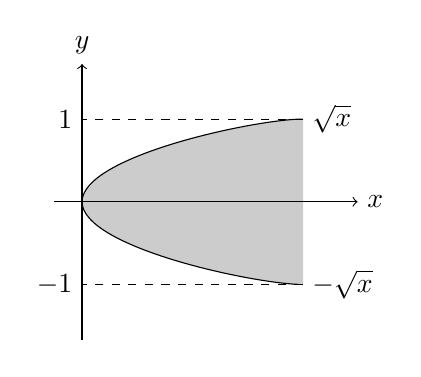
\begin{tikzpicture}[scale=0.7]
		\node [] (0) at (0, 0) {};
		\node [] (1) at (4, 1.5) {};
		\node [] (2) at (4, -1.5) {};
		\node [] (3) at (5, 0) {};
		\node [] (4) at (0, -2.5) {};
		\node [] (5) at (0, 2.5) {};
		\node [] (6) at (-0.5, 0) {};
		\node [] (7) at (0, 1.5) {};
		\node [] (8) at (0, -1.5) {};
		\draw [, in=180, out=90, looseness=0.50, fill=black!20] (0.center) to (1.center);
		\draw [, in=-90, out=180, looseness=0.50, fill=black!20] (2.center) to (0.center);
		

		\draw[color=black!20,fill=black!20] (1.center) to (2.center) to (0.center) to (1.center);
		\draw [dashed] (1.center) to (7.center);
		\draw [->] (6.center) to (3.center) node [anchor=west]{$x$};
		\draw [->] (4.center) to (5.center) node [anchor=south]{$y$};;
		\draw [dashed] (2.center) to (8.center);
		\draw (8.center) node [anchor=east] {$-1$};
		\draw (7.center) node [anchor=east] {$1$};
		\draw (1.center) node [anchor=west] {$\sqrt{x}$};
		\draw (2.center) node [anchor=west] {$-\sqrt{x}$};
\end{tikzpicture}
\end{center}

\[\int\limits_D {fd\mu } \mathop  = \limits_{\begin{array}{*{20}{c}}
 \downarrow \\
 *
\end{array}} \int\limits_{ - 1}^1 {\left( {\int\limits_{x = {y^2}}^1 {fdx} } \right)} dy\]
$$\text{(\textasteriskcentered $=$ Zerlegung des Gebietes in Streifen parallel zur $x-$Achse)}$$
oder mit Zerlegung in Streifen parallel zur $y-$Achse
\[\int\limits_D {fd\mu }  = \int\limits_{x = 0}^1 {\left( {\int\limits_{y =  - \sqrt x }^{y = \sqrt x } {f\left( {x,y} \right)dy} } \right)} dx\]
Manchmal muss man $D$ zerlegen.
\item Bestimme $\int\limits_D {xdxdy} $ wobei $D$ von $y^2=4x$ und $y=2x-4$ begrenzt wird.

\begin{center}
\begin{tikzpicture}[domain=0:10,scale=0.4]
\draw plot[id=x,samples=500] function{2*sqrt(x)} node[anchor=west] {$y=2\sqrt{x}$}; 
\draw plot[id=x,samples=500] function{-2*sqrt(x)} node[anchor=west] {$y=-2\sqrt{x}$};
\draw[->] (0,-8) -- (0,8) node [anchor=south]{$y$};
\draw[->] (0,0) -- (11,0) node [anchor=west]{$x$};
\draw[fill=black] (1,-2) circle (0.15) node [anchor=west]{$~P_1$};
\draw[fill=black] (4,4) circle (0.15) node [anchor=north]{$~~P_2$};
\draw plot[domain=-1:6,id=x,samples=50] function{2*x-4};
\draw (1,3) -- (1,-3);
\draw (1.5,1.5) node {$D$};
\end{tikzpicture}
\end{center}

Schnittpunkte $P_1,P_2$:
\begin{align*}
&4x=y^2=\left( 2x-4\right)^2\\
&\Rightarrow\left( 2x-4\right)^2=4x\dots\\
&\Rightarrow x=1 \text{ und } x=4\\
P_1&=\left(1,-2\right)\hspace{5mm}P_2=\left(4,4\right)
\end{align*}
Zerlegung des Gebiets in Streifen parallel zur $y-$Achse
\[\int\limits_D {xd\mu  = \int\limits_0^1 {\left( {\int\limits_{ - 2\sqrt x }^{2\sqrt x } {xdy} } \right)dx} }  + \int\limits_1^4 {\left( {\int\limits_{y = 2x - 4}^{2\sqrt x } {xdy} } \right)} dx =  \ldots  = 14.4\]
Wenn wir von aussen nach $y$ integrieren, brauchen wir keine Unterteilung
\begin{align*}
\int\limits_D xd\mu  =&\int\limits_{y =  - 2}^{y = 4} {\left( {\int\limits_{y = \frac{{{y^2}}}{4}}^{\frac{y}{2} + 2} {xdx} }\right)dy} \\
 =&\int\limits_{ - 2}^4 {\left( {\left. {\frac{{{x^2}}}{2}} \right|_{\frac{{{y^2}}}{4}}^{\frac{y}{2} + 2}} \right)dy}\\
=&\frac{1}{2}\int\limits_{ - 2}^4 {\left( {{{\left( {\frac{y}{2} + 2} \right)}^2} - \frac{{{y^4}}}{{16}}} \right)dy}
\end{align*}
\end{enumerate}

\subsubsection*{Beispiel für das An dem der Integrationsreihenfolge}
\subsubsection*{Beispiel}
\begin{enumerate}
\item \[\int\limits_0^1 {\int\limits_1^{{e^y}} {f(x,y)dxdy} } \]
$x=1$ und $x=e^y\Rightarrow y=\ln x \Leftrightarrow 1=\ln x \Leftrightarrow x=e$

\begin{center}
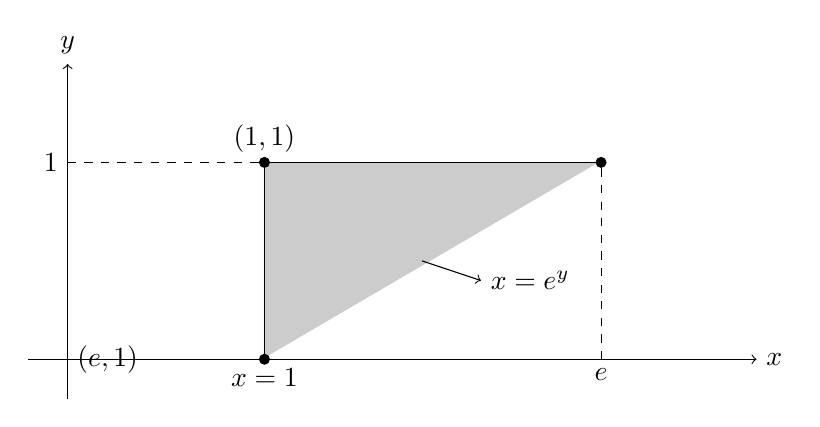
\begin{tikzpicture}[domain=1:2.71,scale=2.5]


\draw[fill=black!20,color=black!20] (1,0)--(1,1) -- (2.71,1) -- cycle;
\draw[thick, color=white] (1,0) --(2.71,1);
\draw[fill=white] plot[id=x,samples=100] function{log(x)} node[anchor=west] {$(e,1)$}; 
\draw[] (1,0)--(1,1) -- (2.71,1);
\draw[fill=black] (1,0) circle (0.025);
\draw[fill=black] (1,1) circle (0.025);
\draw[fill=black] (2.71,1) circle (0.025);
\draw (1,1) node [anchor=south]{$(1,1)$};
\draw[->] (0,-0.2) --(0,1.5) node [anchor=south]{$y$};
\draw[->] (-0.2,0) --(3.5,0) node [anchor=west]{$x$};
\draw (2.1,0.4) node [anchor=west]{$x=e^y$};
\draw[dashed] (2.71,0)--(2.71,1);
\draw (2.71,0) node [anchor=north]{$e$};
\draw (1,0) node [anchor=north]{$x=1$};
\draw[dashed] (0,1)--(1,1);
\draw (0,1) node [anchor=east]{$1$};
\draw[->] (1.8,0.5) --(2.1,0.4);
\end{tikzpicture}
\end{center}

\[\int\limits_1^e {\int\limits_{y = \log x}^{y = 1} {f(x,y)dydx} } \]

\begin{center}
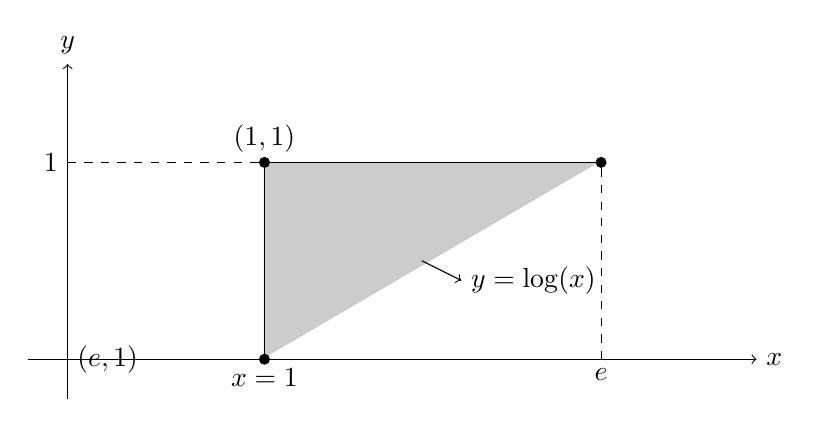
\begin{tikzpicture}[domain=1:2.71,scale=2.5]


\draw[fill=black!20,color=black!20] (1,0)--(1,1) -- (2.71,1) -- cycle;
\draw[thick, color=white] (1,0) --(2.71,1);
\draw[fill=white] plot[id=x,samples=100] function{log(x)} node[anchor=west] {$(e,1)$}; 
\draw[] (1,0)--(1,1) -- (2.71,1);
\draw[fill=black] (1,0) circle (0.025);
\draw[fill=black] (1,1) circle (0.025);
\draw[fill=black] (2.71,1) circle (0.025);
\draw (1,1) node [anchor=south]{$(1,1)$};
\draw[->] (0,-0.2) --(0,1.5) node [anchor=south]{$y$};
\draw[->] (-0.2,0) --(3.5,0) node [anchor=west]{$x$};
\draw (2,0.4) node [anchor=west]{$y=\log(x)$};
\draw[dashed] (2.71,0)--(2.71,1);
\draw (2.71,0) node [anchor=north]{$e$};
\draw (1,0) node [anchor=north]{$x=1$};
\draw[dashed] (0,1)--(1,1);
\draw (0,1) node [anchor=east]{$1$};
\draw[->] (1.8,0.5) --(2,0.4);
\end{tikzpicture}
\end{center}

\item Berechne \[\int\limits_0^1 {\int\limits_x^1 {{e^{{y^2}}}dydx} } \] Man kann das Integral $\int\limits_a^b {{e^{{y^2}}}dydx} $ nicht direkt berechnen, weil man kein explizit Stammfunktion für $e^{y^2}$ finden kann. Man kann sich die Reihenfolge der Zerlegung beliebig heraussuchen damit die Rechnung möglichst einfach wird. 

\begin{center}
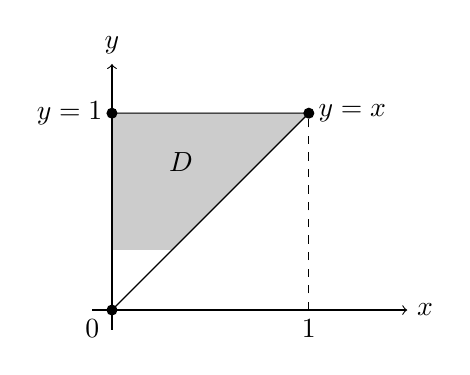
\begin{tikzpicture}[scale=2.5]
\draw[fill=black!20,color=black!20] (0,0)--(1,1)--(0,1)--cycle;
\draw[fill=white,color=white] (0,0)--(1,0)--(1,0.3) -- (0,0.3)--cycle;
\draw[] (0,0)--(1,1)--(0,1);
\draw[->] (-0.1,0) -- (1.5,0) node [anchor=west]{$x$};
\draw[->] (0,-0.1) -- (0,1.25) node [anchor=south]{$y$};

\draw [dashed] (1,0)--(1,1) node [anchor=west]{$y=x$};
\draw[fill=black] (1,1) circle (0.025);
\draw[fill=black] (0,0) circle (0.025);
\draw[fill=black] (0,1) circle (0.025);

\draw (1,0) node [anchor=north]{1};
\draw (-0.1,0) node [anchor=north]{0};

\draw (0.35,0.75) node[] {$D$};
\draw (0,1) node[anchor=east] {$y=1$};
\end{tikzpicture}
\end{center}

\begin{align*}
\int\limits_{x = 0}^{x = 1} {\int\limits_{y = x}^{y = 1} {{e^{{y^2}}}dydx} }  &= \int\limits_{y = 0}^{y = 1} {\int\limits_{x = 0}^{x = y} {{e^{{y^2}}}dxdy} } \\
 &= \int\limits_0^1 {\left[ {\left. {x{e^{{y^2}}}} \right|_{x = 0}^{x = y}} \right]} dy\\
 &= \int\limits_0^1 {y{e^{{y^2}}}dy}  = \left. {\frac{{{e^{{y^2}}}}}{2}} \right|_0^1 = \frac{1}{2}\left( {e - 1} \right)
\end{align*}
\end{enumerate}

\subsubsection*{Bemerkung 9.13}
\begin{enumerate}
\item Das Integral \[A = \int\limits_D {1d\mu } \] ergibt die Fläche von $D$. Für einen Normalbereich bzgl. der $x-$Achse erhalten wir daraus die bekannte Formel
\[A = \int\limits_a^b {\int\limits_{g(x)}^{h(x)} {1dydx} }  = \int\limits_a^b {\left( {h(x) - g(x)} \right)dx} \]

\begin{center}
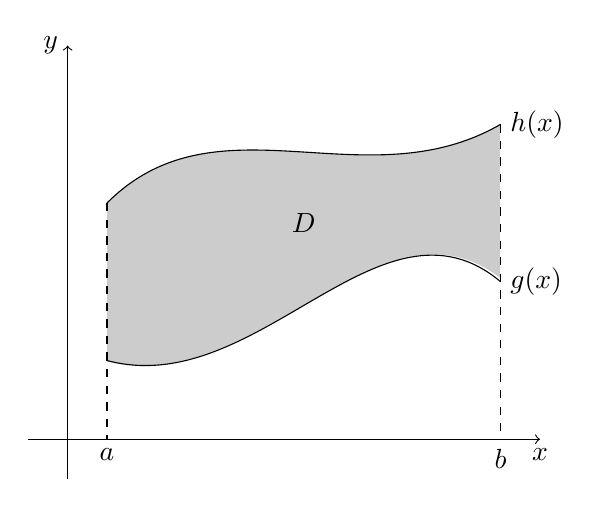
\begin{tikzpicture}[scale=1]
\shade[top color=black!20,bottom color=black!20,in=-150, out=45] 
      (0.5,3) to (5.5,4) |- (0.5,0);
\shade[top color=white,bottom color=white,in=140, out=-15] 
      (0.45,1) to (5.55,2) |- (0.5,0);

\draw[->] (-0.5,0)--(6,0) node [anchor=north]{$x$};;
\draw[->] (0,-0.5)--(0,5) node [anchor=east]{$y$};
\draw [in=-150, out=45] (0.5,3) to (5.5,4);
\draw [in=140, out=-15] (0.5,1) to (5.5,2);
\draw[dashed] (0.5,3)--(0.5,0) node [anchor=north]{$a$};
\draw[dashed] (5.5,4)--(5.5,0) node [anchor=north]{$b$};
\draw (5.5,2) node [anchor=west]{$g(x)$};
\draw (5.5,4) node [anchor=west]{$h(x)$};
\draw (3,2.75) node []{$D$};
\end{tikzpicture}
\end{center}

\item Interpretiert man $\rho(x,y)$ als ortabhängige Flächendichte, so erhält man mit \[m = \int\limits_D {\rho \left( {x,y} \right)d\mu } \] die Masse von $D$
\end{enumerate}

\begin{definition}{9.14}
Eine Teilmenge $D\subset\R^3$ heisst Normalbereich, falls es eine Darstellung
\[D = \left\{ {\left. {\left( {x,y,z} \right) \in {R^3}} \right|a \le x \le b;g(x) < y < h(x);\varphi \left( {x,y} \right) \le z \le \psi \left( {x,y} \right)} \right\}\] gibt.\\

(Vertauscht man die Rollen von $x,y$ und $z$ so entstehen weitere Mengen, die auch Normalbereiche genannt werden.)
\end{definition}

\subsubsection*{Satz 9.15}
Sei $D\subset\R^3$ ein Normalbereich mit Darstellung wie oben, und $f:D\to\R$ stetig. Dann gilt \[\int\limits_D {fd\mu }  = \int\limits_a^b {\int\limits_{g(x)}^{h(x)} {\int\limits_{\varphi \left( {x,y} \right)}^{\psi \left( {x,y} \right)} {f\left( {x,y,z} \right)dzdydx} } } \]
\missingfigure{Page 228, middle}
$z=\varphi \left( {x,y} \right)$ und $z=\psi \left( {x,y} \right)$ stellen die ``Grund-'' und Deckelfläche von $D$ dar. \\

Der Normalbereich $A$ ist die senkrechte Projektion von $D$ in die $x-y$ Ebene. Dessen ``Grund-'' und ``Deckelkurve'' sind durch $y=g(x)$ und $y=h(x)$ gegeben.

\subsubsection*{Bemerkung 9.16}
Das Integral
\[ V=\int\limits_D 1 d\mu\text{ für }D\subset\R^3\]
ergibt das Volumen von $D$. Für einen Normalbereich
\[D = \left\{ {\left( {x,y,z} \right)\mid a \le x \le b,g(x) \le y \le h(x),\varphi \left( {x,y} \right) \le z \le \psi \left( {x,y} \right)} \right\}\]
 erhält man
\[V = \int\limits_a^b {\int\limits_{g(x)}^{h(x)} {\int\limits_{\varphi \left( {x,y} \right)}^{\psi \left( {x,y} \right)} {1dzdydx} } }  = \int\limits_a^b {\int\limits_{g(x)}^{h(x)} {\psi \left( {x,y} \right) - \varphi \left( {x,y} \right)dydx} } \]

\section{Substitutionsregel}
Häufig sind kartesische Koordinaten für die Berechnung von Integralen eher ungeignet. z.B. wenn man Symmetrien bezüglich gewisser Punkte oder Achsen ausnutzen will.\\

Wir behandeln als nächstes Variablentransformationen vom Typ $\Phi:\R^n\to\R^n$ und verallgemeinern die eindimensionale Substitutionsregel:
\[\int\limits_{\varphi (a)}^{\varphi (b)} {f(x)dx}  = \int\limits_a^b {f\left( {\varphi \left( t \right)} \right)\varphi '\left( t \right)dt} \]
mit $f$ stetig, $x=\varphi\left( t\right)$ $\varphi :\lbrack a,b\rbrack\to I$ stetig differenzierbar, $I=$ Intervall. Zunächst erinnern wir uns an die lineare Algebra:\\

Das Bild des Einheitsquadrats/-würfels unter der linearen Abbildung
\begin{align*}
\Phi:\R^n&\to\R^n\\
\vec x&\to A\vec x\hspace{5mm}A\in\R^{n\times n}
\end{align*}
ist ein Parallelogramm mit Fläche $\left| \det A\right|$

\begin{center}
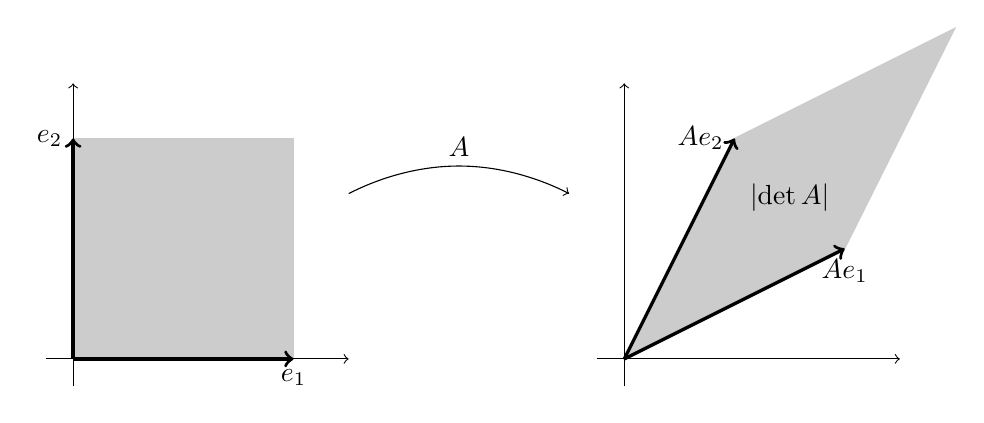
\begin{tikzpicture}[scale=0.7]
\draw[fill=black!20,color=black!20] (0,0) --(0,4) --(4,4) --(4,0)--cycle;
\draw[fill=black!20,color=black!20] (10,0) --(12,4) --(16,6) --(14,2)--cycle;
\draw[->] (-0.5,0)--(5,0);
\draw[->] (0,-0.5)--(0,5);
\draw[->,very thick] (0,0)--(0,4) node [anchor=east]{$e_2$};
\draw[->,very thick] (0,0)--(4,0) node [anchor=north]{$e_1$};
\draw[->] (5,3) parabola bend(7,3.5) (9,3);
\draw (7,3.5) node [anchor=south]{$A$};

\draw[->] (10-0.5,0)--(10+5,0);
\draw[->] (10+0,-0.5)--(10+0,5);
\draw[->,very thick] (10+0,0)--(10+2,4) node [anchor=east]{$Ae_2$};
\draw[->,very thick] (10+0,0)--(10+4,2) node [anchor=north]{$Ae_1$};
\draw (13,2.5) node [anchor=south]{$\left| \det A\right|$};

\end{tikzpicture}
\end{center}

Dies bleibt wahr, wenn man zur affin-linearen Abbildung $\Phi\left(\vec{x}\right)=A\vec a+\vec b$ betrachtet, es kommt ja nur ein Verschiebung dazu
\missingfigure{Page 231 bottom}
Nun betrachten wir eine differenzierbare nichtlineare Transformation $\Phi:\R^n \to\R^n$. Dann gilt, zumindest nahe eines festen Punktes $\vec x\in\R^n$:
\[ \Phi\left( x\right)\approx\Phi\left( x_0\right) + d\Phi\left( x_0\right) \left( \vec{x}-\vec{x_0}\right)\]
Die rechte Seite stellt gerade eine Abbildung vom Typ $A\vec x+\vec b$ dar, wobei die Jacobi-Matrix $d\Phi\left( x_0\right)\in\R^n\times\R^n$ die Rolle von $A$ (und $\Phi\left( x_0\right)$ von $\vec b$) übernimmt. Damit ist der lokale Flächenverzerrungsfaktor von $\Phi$ gegeben durch $\left| \det d\Phi\left( x_0\right)\right|$ d.h. den Betrag der Jacobi- oder Funktionaldeterminante. Die lokale Flächenverzerrung muss bei der Substitution in Integralen berücksichtigt werden und zwar in der Form
\[``d\vec x = \left| {\det d\Phi \left( {\vec y} \right)} \right|d\vec{y} \text{ ''},{\text{ falls }}\vec x = \Phi \left( y \right)\]
Geometrische Darstellung in $\R^2$
\missingfigure{Page 232.5 top}
Die Flächen der einander entsprechenden markierten Vierecke unterscheiden sich gerade um den Faktor $\left|\det d\Phi\left( x_1\right)\right|$ bzw. $\left|\det d\Phi\left( x_2\right)\right|$
\subsection*{Substitutionsregel}
\subsubsection*{Satz 9.17}
Sei $U,V\subset\R^n$ offen, $\Phi:U\to V$ bijektiv, stetig diff., $\det d\Phi\left( \vec y\right)\not=0$ $\forall\vec y\in U$, sowie $f: V\to\R$ stetig. Dann gilt
\[\int\limits_V {f\left( {\vec x} \right)d\mu \left( {\vec x} \right)}  = \int\limits_{\Phi \left( U \right) = V} {f\left( {\Phi \left( {\vec y} \right)} \right)\left| {\det d\phi \left( y \right)} \right|} d\mu \]

\subsubsection*{Beispiel 9.18}
\begin{enumerate}
\item Berechne $\iiint\limits_V d\mu$, wobei \[\mathop {\text{V}}\limits_{\begin{array}{*{20}{c}}
 \downarrow \\
{{\text{Kugeloktanten}}}
\end{array}} {\text{ = }}\left\{ {\left. {{{\left( {x,y,z} \right)}^t}} \right|{x^2} + {y^2} + {z^2} \le 1,x,y,z \ge WHAT} \right\}\] \todo{chopped content, page 233 middle to bottom}Es ist einfacher in Kugelkoordinaten zu rechnen
\[\Phi \left( {r,\theta ,\psi } \right) = \left( {\begin{array}{*{20}{c}}
{r\cos \theta \cos \psi }\\
{r\sin \theta \cos \psi }\\
{r\sin \psi }
\end{array}} \right)\]
Die Transformation $\Phi$ ist auf ganz $\R^3$ definiert und mit \[U = \left[ {0,1} \right] \times \left[ {0,\frac{\pi }{2}} \right] \times \left[ {0,\frac{\pi }{2}} \right]\]
gilt
\begin{align*}
\Phi\left( U\right) =&V\\
\det\left( d\Phi\right)=&r^2\cos\psi\\
\text{vol}\left(V\right)=&\int\limits_{V} d\mu\left( \vec x\right)=\int\limits_0^1\int\limits_0^{\frac{\pi}{2}}\int\limits_0^{\frac{\pi}{2}} r^2\cos\psi d\psi d\theta dr=\frac{\pi}{2}
\end{align*}
\item Berechne das Integral
\[ \iint\limits_D x dx dy\text{ wobei $D=$Viertelkreis}\]
\begin{align*}
\int\limits_{x = 0}^1 {\int\limits_{y = 0}^{\sqrt {1 - {x^2}} } x } dydx =&\int\limits_0^1 {\left( {\left. {xu} \right|_0^{\sqrt {1 - {x^2}} }} \right)dx} \\
=&\int\limits_0^1 x\sqrt{1-x^2}dx\\
=&\int\limits_0^1 {\frac{{{u^{{1 \mathord{\left/
 {\vphantom {1 2}} \right.
 \kern-\nulldelimiterspace} 2}}}}}{2}} du =  - \frac{1}{2} \cdot \left. {\frac{{{u^{{3 \mathord{\left/
 {\vphantom {3 2}} \right.
 \kern-\nulldelimiterspace} 2}}}}}{{{3 \mathord{\left/
 {\vphantom {3 2}} \right.
 \kern-\nulldelimiterspace} 2}}}} \right|_0^1\\
=&-\frac{1}{3}
\end{align*}
mit $1-x^2=u$, $-2xdx=du$\\
\underline{Oder:}\\
\[ \iint\limits_D x dx dy \hspace{10mm}\left( {\begin{array}{*{20}{c}}
x\\
y
\end{array}} \right) = \mathop {\left( {\begin{array}{*{20}{c}}
{r\cos \theta }\\
{r\sin \theta }
\end{array}} \right)}\limits_{dxdy = rdrd\theta } \]

\begin{align*}
\int\limits_0^{\pi /2} {\int\limits_0^1 {{r^2}\cos \theta drd\theta } }  =&\int\limits_0^{\pi /2} {\cos \theta \left( {\left. {\frac{{{r^3}}}{3}} \right|_0^1} \right)d\theta } \\
 =&\frac{1}{3}\int\limits_0^{\pi /2} {\cos \theta d\theta }  = \left. { - \frac{1}{3}\sin \theta } \right|_0^{\pi /2} =  - \frac{1}{3}
\end{align*}
\item Die Substitutionsregel in mehreren Variablen ist manchmal auch nützlich zur Berechnung von Integralen in einer Variable. Zunächst möchten wir das Integral \[ I=\int\limits_0^\infty e^{-x^2} dx\] berechnen. Wir berechnen $I$ durch Berechnung eines Flächenintegrals wie folgt. Es gilt
\begin{align*}
{I^2} =&{\left( {\int\limits_0^\infty  {{e^{ - {x^2}}}dx} } \right)^2}\\
 =&\mathop {\lim }\limits_{R \to \infty } \left( {\int\limits_0^R {{e^{ - {x^2}}}dx} } \right)\left( {\int\limits_0^R {{e^{ - {y^2}}}dy} } \right)\\
 =&\mathop {\lim }\limits_{R \to \infty } {I_R}
\end{align*}
für \[{I_R} = \int\limits_{\left[ {0,R} \right] \times \left[ {0,R} \right]} {{e^{ - \left( {{x^2} + {y^2}} \right)}}dxdy} \]
Bezeichnet $K_\rho$ den Viertelkreis im 1. Quadrant mit Radius $r$, so gilt
\[\int\limits_{{K_R}} {{e^{ - \left( {{x^2} + {y^2}} \right)}}dxdy \le {I_R}\int\limits_{{K_{\sqrt 2 R}}} {{e^{ - \left( {{x^2} + {y^2}} \right)}}dxdy} } \]
\missingfigure{Page 236 bottom}
Die Integrale über $K_\rho$ berechnet man nun über Polarkoordinaten
\[\int\limits_{{K_\rho }} {{e^{ - \left( {{x^2} + {y^2}} \right)}}dxdy}  = \int\limits_0^\rho  {\int\limits_0^{\pi /2} {{e^{ - {r^2}}}rdrd\theta } }  = \frac{\pi }{4}\left( {1 - {e^{{\rho ^2}}}} \right)\]
und somit gelten die Abschätzungen
\[\frac{\pi }{4}\left( {1 - {e^{ - {R^2}}}} \right) \le {I_R} \le \frac{\pi }{4}\left( {1 - {e^{ - 2{R^2}}}} \right)\]
und es gilt schliesslich
\[\mathop {\lim }\limits_{R \to \infty } {I_R} = \frac{\pi }{4}\]
d.h. \[{I^2} = \mathop {\lim }\limits_{R \to \infty } {I_R} = \frac{\pi }{4}\]
d.h. \[I = \frac{{\sqrt \pi  }}{2} = \int\limits_0^\infty  {{e^{ - {x^2}}}dx} \]
\end{enumerate}

\section{Der Satz von Green}
Wir erinnern uns: Sei $\Omega\subset\R^2$, ist $V:\Omega\to\R^2$ ein $C'-$Vektorfeld mit Potential $f$, so folgt
\[\rot\left( v(x)\right)=\rot\left( \nabla f(x)\right)=0\hspace{10mm}\forall x\in\R^2 \]
wobei
\[\rot\left( v\left( x,y\right)\right)=\frac{\partial v_2}{\partial x}\left( x,y\right) -\frac{\partial v_1}{\partial y}\left( x,y\right)\]
so ist
\[\rot v=\frac{\partial v_2}{\partial x} -\frac{\partial v_1}{\partial y}=0 \]
in wei Dimensionen eine notwendige Bedingung für die Existenz eines Potentials.\\

Die Bedingung $\rot(v)=0$ ist sogar eine hinreichende Bedingung, falls das Gebiet $\Omega$ einfach zusammenhängend ist. In diesem Fall
\[\oint\limits_\gamma  v  = \int\limits_\gamma  {\nabla fds = f\left( {\gamma \left( 1 \right)} \right) - } f\left( {\gamma \left( 0 \right)} \right) = 0\]
für alle geschlossene Weg $\gamma$ und für einen nichtgeschlossenen Weg $\gamma$
\missingfigure{Add picture on 238 bottom and 239 top side by side}
\[\int\limits_\gamma  v  = \int\limits_\gamma  {\nabla fds = f\left( {\gamma \left( 1 \right)} \right) - } f\left( {\gamma \left( 0 \right)} \right)\]
d.h. falls das Vektorfeld ein Gradientenfeld ist, ist das Integral $\int\limits_\gamma  v $ eine Funktion der Endpunkte. \\

Anders gesagt, es gibt Fälle wo ein Wegintegral (d.h. ein Integral auf einem eindimensionalen Objekt mithilfe einer 0-dimensionalen Menge) berechnet werden kann.

\subsubsection*{Bemerkung}
Auch für Funktionen einer Variable: Falls $F'=f$ ist, dann gilt \[\int\limits_a^b {f(x)dx}  = F\left( b \right) - F\left( a \right)\] Hauptsatz der Integralrechnung einer Variable

\subsubsection*{Frage}
Gibt es auch Fälle wo ein zweidimensionales Integral mithilfe einer eindimensionalen Menge berechnet werden kann?\\

\noindent Die Antwort ist genau der Inhalt des Satzes von Green

\subsubsection*{Satz 9.19 (Green)}
Sei $\Omega \in\R^2$ ein Gebiet, dessen Rand $\partial\Omega$ eine stückweise $C'$ Parameterdarstellung hat. Sei $U$ eine offene Menge mit $\Omega\subset U$ und sei
\[ f=\frac{\partial Q}{\partial x}\left( x,y\right) -\frac{\partial P}{\partial y}\left( x,y\right) \]
wobei $P,Q\in C'\left( U\right)$. Dann gilt
\[ \iint\limits_\Omega \left(\frac{\partial Q}{\partial x}-\frac{\partial P}{\partial y}\right)d\mu = \int\limits_{\partial \Omega } {Pdx + Qdy} \]
wobei $\partial \Omega$ so parametrisiert wird, dass $\Omega$ zur Linken des Randes liegt. \\

\noindent\underline{Anders gesagt:}\\

\noindent Sei $V=\left( P,Q\right)$ ein $C'$ Vektorfeld auf dem Gebiet $U$. Sei $\Omega\subset U$ ein Gebiet, dessen rand $\partial\Omega$ ein Stückweise $C'$ Parameterdarstellung hat. Die parametrisierung von $\Omega$ sei so gewählt dass $\Omega$ stets links zur Durchlaufrichtung liegt. Dann gilt
\[\int\limits_{\partial \Omega } {Vds}  = \int\limits_{\partial \Omega } {Pdx + Qdy}  = \iint\limits_\Omega \rot\left( V \right)d\mu \]
Bevor wir die Idee des Beweises geben, geben wir einige Beispiele und Anwendungen

\subsubsection*{Beispiel 9.20}
\begin{enumerate}
\item Wir betrachten das Vektorfeld \[ F\left( x,y\right) = \left( y+3x,y-2x\right) \]
und wir möchten dieses Kraftfeldes entlang der im Gegenuhrzeigersinn durchlaufenen Ellipse $\gamma: 4x^2+y^2=4$ bestimmen. Die Arbeit ist
\begin{align*}
\int\limits_\gamma  {Fd\vec s}  =&\int\limits_\gamma  {Pdx + Qdy} \\
 =&\int\limits_\gamma  {\left( {y + 3x} \right)dx + \left( {2y - x} \right)dy} \\
{\text{Green }} \to {\text{ }} =&\iint\limits_\Omega\frac{{\partial \left( {2y - x} \right)}}{{\partial x}} - \frac{{\partial \left( {y + 3x} \right)}}{{\partial y}}\\
=&\iint -1-1d\mu=-2\iint\limits_\Omega d\mu\\
=&-2\cdot\text{(Flächeninhalt von Ellipse $4x^2+y^2=4$)}\\
\end{align*}
\todo[inline]{Can't understand the result, page 242 top}
\missingfigure{Page 243, bottom}
\item Berechne das Wegintegral \[\int\limits_{\partial \Omega } {\left( {5 - xy - {y^2}} \right)dx - \left( {2xy - {x^2}} \right)dy} \] wobei $\Omega$ das Quadrat mit Eckpunkten $(0,0),(0,1),(1,1),(1,0)$ im Gegenuhrzeigersinn ist
\begin{align*}
&\int\limits_{\partial A} {\left( {5 - xy - {y^2}} \right)dx - \left( {2xy - {x^2}} \right)dy} \\
=&\iint\limits_\Omega\left[ {\frac{\partial }{{\partial x}}\left( {2xy - {x^2}} \right) - \frac{\partial }{{\partial y}}\left( {5 - xy - {y^2}} \right)} \right]d\mu \\
=&\iint\limits_\Omega\left(  2y-2x\right) - \left( -x-2y\right) d\mu\\
=&3\iint\limits_\Omega d\mu=\int\limits_0^1\int\limits_0^1 x dx dy=\frac{3}{2}
\end{align*}
\item Mittels des Satzes von Green können wir den Flächeninhalt eines Gebiets mithilfe eines Wegintegrals berechnen. Und zwar
\[ \text{Flächeninhalt$\left( \Omega\right)$}=\iint\limits_\Omega d\mu=\iint\left( \frac{\partial Q}{\partial x}-\frac{\partial P}{\partial y}\right) d\mu\]
wobei $P$ und $Q$ Funktionen mit $\frac{\partial Q}{\partial x}-\frac{\partial P}{\partial y}=1$ sind. Zum Beispiel können wir
\begin{align*}
Q\left( x,y\right)=&\frac{1}{2}x\\
P\left( x,y\right)=&-\frac{1}{2}x
\end{align*}
nehmen. Daraus folgt, dass \[ F\left( \Omega\right) = \frac{1}{2}\int\limits_{\partial\Omega}-y dx+xdy\]
Als ein Beispiel können wir verifizieren dass der Flächeninhalt des Kreises $x^2+y^2\leq 4$ gleich $4\pi$ ist. \\

Betrachte die Parameterdarstellung $\gamma\left(\theta\right)=\left( 2\cos\theta,2\sin\theta\right)$, $\theta\in\lbrack 0,2\pi\rbrack$ des Randes $\partial\Omega$
\begin{align*}
F\left(\Omega\right)=&\iint\limits_\Omega d\mu = \frac{1}{2}\int\limits_{\partial\Omega} -ydx+xdy\\
=&\frac{1}{2}\int\limits_0^{2\pi}\left( -2\sin\theta\right)\left( -2\sin\theta\right) + \left( 2\cos\theta\right)\left( 2\cos\theta\right) d\theta\\
=&\frac{1}{2}\int\limits_0^{2\pi}4\left( \sin^2\theta+\cos^2\theta\right)d\theta=2\cdot 2\pi=4\pi
\end{align*}
\end{enumerate}
